
\section{Cross validation}
\label{sec:model_development_process}
The aim of developing a manoeuvring model with parameter estimation is to develop a model that can generalize outside the known data. The method presented in this thesis is assessed with the hold-out evaluation \cite{sammut_holdout_2017}. The data in this evaluation is divided into three sets: the training set, the validation set, and the test set as seen in \autoref{fig:model_development_process}.

\begin{figure}[H]
\centering
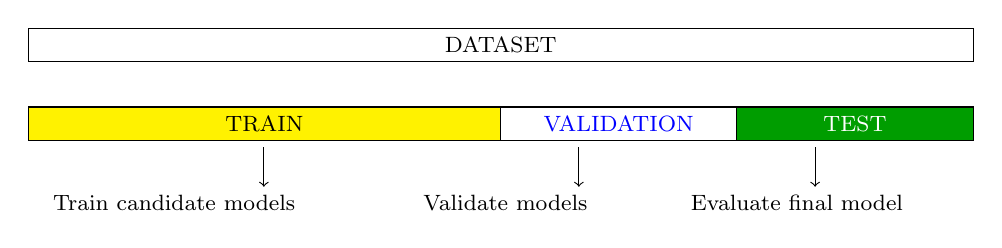
\begin{tikzpicture}

\node (dataset)[rectangle,
    anchor=west,
    draw,
    text = black,
    minimum width=12cm,
    fill = white] at (0, 0) {\footnotesize DATASET};

\node (train)[rectangle,
    draw,
    anchor=west,
    text = black,
    minimum width=6cm,
    fill = yellow] at (0, -1cm) {\footnotesize TRAIN};

\node (validation)[rectangle,
    draw,
    anchor=west,
    text = blue,
    minimum width=3cm,
    fill = white] at (6cm, -1cm) {\footnotesize VALIDATION};

\node (test)[rectangle,
    draw,
    anchor=west,
    text = white,
    minimum width=3cm,
    fill = black!15!green!255] at (9cm, -1cm){\footnotesize TEST};
    
\node (train_multiple)[rectangle,
    draw,
    anchor=west,
    text = black,
    draw = none,
    fill = none] at (0.2cm, -2cm){\footnotesize Train candidate models};
    
\node (validate_models)[rectangle,
    draw,
    anchor=west,
    text = black,
    draw = none,
    fill = none] at (4.9cm, -2cm){\footnotesize Validate models};
    
\node (evaluate_models)[rectangle,
    draw,
    anchor=west,
    text = black,
    draw = none,
    fill = none] at (8.3cm, -2cm) {\footnotesize Evaluate final model};

\draw[->] (3,-1.3) -- (3,-1.8);
\draw[->] (7,-1.3) -- (7,-1.8);
\draw[->] (10,-1.3) -- (10,-1.8);



\end{tikzpicture}
\caption{Model development process with hold-out evaluation.}
\label{fig:model_development_process}
\end{figure}

\noindent The purpose of the training set is to train all the candidate models using the proposed parameter estimation method. The validation set is used to select the most effective candidate model. The training and validation sets are joined to train the selected model as the final model. The final model is used for predicting the test set, which is used to evaluate the accuracy of the model. These three sets are not divided randomly;  they are divided to assess the model’s extrapolation ability. The data sets are therefore split to have the smallest yaw rates, drift-angles, and rudder-angles in the training set; the medium values in the validation set; and the largest values in the test set.
Examples of this can be seen for the two test cases in this thesis in \autoref{fig:kvlcc2_datasets} and  \autoref{fig:wpcc_datasets} in the next chapter.